Jupyter works in a REPL-like fashion, we give a brief introduction here for a more detailed introduction we refer the interested reader to \cite{jupyter-doc:on}. 
Notebooks consist of a set of cells; each of which contains either rich text or code that can be evaluated. 
The Jupyter user interface is implemented using TypeScript in the browser, the backend is implemented in Python and delegates the programming-language specific features to so-called kernels via a networking protocol. 
Each kernel works exactly like a REPL, that is to say they receive the user input of the code cells and produce output that should be presented to the user. 
Additionally, kernels can implement custom interactions using widgets, consisting of re-usable user interface components that communicate directly with the kernel.  
Kernels for a specific programming language are typically implemented in that programming language, to ease implementation and make use of existing tool support. 

We designed and implemented a Jupyter kernel for MMT. 
The source code is available at \cite{mmt_jupyter:on}. 
We describe its interface in Section~\ref{sec:kernel:syntax}, the implementation in Section~\ref{sec:kernel:impl} and our conversion between MMT datastructures and notebook in Section~\ref{sec:kernel:mapping}.
In Section~\ref{sec:kernel:widgets}, we describe and discuss our implementation of widgets within our kernel. 

\subsection{Interface}\label{sec:kernel:syntax}

MMT differs from typical computational engines in Jupyter in that it does not only (and not even primarily) perform computation but also handles symbolic expressions with uninterpreted function symbols, whose semantics is described by logical axioms.
Another important difference is how MMT handles context and background knowledge.
Kernels for (mathematics-oriented or general purpose) programming languages, as typical in Jupyter, build and maintain a dynamic context of declarations with imperative assignment and stack-oriented shadowing and rely on a fixed --- often object-oriented --- background library of computational functionality.
MMT, on the other hand, uses graphs of inter-connected theories to represent a multitude of possible contexts and background libraries and to move knowledge between contexts.
To adequately handle these subtleties, we systematically specified a new interface for Jupyter-style interactions with MMT.

\paragraph{Sessions}
On top of the notebook abstraction, Jupyter interactions are managed in \textbf{sessions}: every browser page opening a notebook creates a new session.

MMT already has an abstraction that can closely model a notebook, called a document \ednote{CITATION}. 
In MMT terms, a document is a narrative construct that contains a set of declarations. 
Each input within the Jupyter session can be represented as a single declaration within the document; see Section~\ref{sec:kernel:mapping} for further applications of this mapping. 

Thus it makes sense to represent each session as an ephemeral\footnote{We call an MMT document \textbf{ephemeral}, iff it is (at least initially; it can be serialized and saved) created only in memory in the MMT process; apart from this, it behaves like any other MMT document}) MMT document. 
This gives each session a unique MMT URI, which in turn allows full referencing of all document components.
All commands executed within a session manipulate the associated document, most importantly by interactively creating new theories and then calling MMT algorithms on them.
The latter include but are not limited to computation.

\paragraph{Input}
The possible inputs accepted by the MMT kernel are divided into three groups.
\begin{itemize}
\item \textbf{Global management commands} allow displaying and deleting all current sessions.
 In practice, these commands are typically not available to common users, which should only have access to their own session.
\item \textbf{Local management commands} allow starting, quitting, and restarting the current session. These are the main commands issued by the frontend in response to user action.
\item \textbf{Content commands} are the mathematically meaningful commands and described below.
\end{itemize}

The content commands are again divided into three groups:
\begin{itemize}
 \item \textbf{Write-commands} send new content to the MMT backend to build the current MMT document step by step.
   The backend maintains one implicit, ephemeral MMT document for each session, and any write command changes that document.
 \item \textbf{Read-commands} retrieve information from the backend without changing the session's document.
   These include lookups (both in the session document and in any other accessible document) or computations.
  \item \textbf{Interactive-commands} that create a new user interface component allowing the user to interactively read and write MMT content. 
   In the Jupyter system these are implemented as so-called widgets, and technically break the REPL-paradigm. 
   We will not discuss these now; instead we will discuss them in more detail below in Section~\ref{sec:kernel:widgets}. 
\end{itemize}

A write-command typically consists of a single MMT declaration roughly corresponding to a line in a typical MMT source file.
However, the nesting of declarations is very important in MMT.
This is in contrast to many programming language kernels where nesting is often optional, e.g., to define new functions or classes;
for many current kernels, it makes sense to simplify the implementation by requiring that the entire top-level command, including any nesting, be contained in a single cell.

In our MMT kernel, all declarations that may contain nested declarations (most importantly all MMT documents and theories) are split into parts as follows: the header, the list of nested declarations, and a special end-of-nesting marker.
Each of these is communicated in a separate write-command.
The semantics of MMT is carefully designed in such a way that \emph{i}) any local scope arising from nesting has a unique URI, and \emph{ii}) if a well-formed MMT document is built incrementally by appending individual declarations to a currently open local scope, any intermediate document is also well-formed.
This is critical to make our implementation feasible: the MMT kernel maintains the current document as well as the URI of the current scope; any write-command affects the current scope, possibly closing it or creating new subscopes.
This ensures that all nested declarations are parsed and interpreted in the right scope.

\begin{wrapfigure}{l}{7.5cm}
  \vspace{-20pt}
  \begin{minipage}[c]{4cm}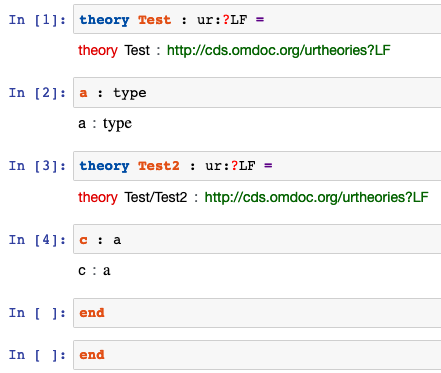
\includegraphics[width=4cm]{screenshots/nesting}\end{minipage}
  \begin{minipage}[c]{3cm}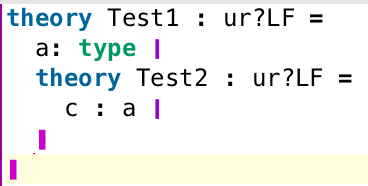
\includegraphics[width=3cm]{../D4.11/test_theory}\end{minipage}
  \caption{Content Commands for Building Theory Graphs}\label{fig:test_theory}
  \vspace{-20pt}
\end{wrapfigure}

For example, the sequence of commands on the left of Figure~\ref{fig:test_theory} builds two nested theories, where the inner one refers to the type \texttt{a} declared in the outer one.
The right-hand side of Figure~\ref{fig:test_theory} shows the equivalent MMT surface syntax on the right.
Semantically, there is no difference between entering the left-hand side interactively via our new kernel or processing the write commands on the right with the standard MMT parser.

An additional special write-command is \texttt{eval T}.
It interprets \texttt{T} in the current scope, infers its type \texttt{A}, computes its value \texttt{V}, and then adds the declaration \texttt{resI:A=V} to the current theory, where \texttt{I} is a running counter of unnamed declarations.
This corresponds most closely to the REPL functionality in typical Jupyter kernels.

While write-commands correspond closely to the available types of MMT declarations, the set of read-commands is extensible.
For example, the commands \texttt{get U} where \texttt{U} is any MMT URI returns the MMT declaration of that URI.

\paragraph{Output}
The kernel returns the following kinds of return messages:
\begin{itemize}
\item \textbf{Admin messages} are strings returned in response to session management commands.
\item \textbf{New-element messages} return the declaration that was added by a write-command.
\item \textbf{Existing-element messages} return the declaration that was retrieved by a \texttt{get} command.
\end{itemize}
Like read-commands, the set of output messages is extensible.

The new-element and existing-element messages initially return the declaration in MMT's abstract syntax.
And a post-processing layer specific to Jupyter renders them in HTML+presentation MathML.
That way, the core kernel functionality can be reused easily in other frontends than Jupyter.

\subsection{Implementation}\label{sec:kernel:impl}

Generally, Jupyter emphasizes protocols that specify the communication between frontend and backend. 
% Recall that the frontend is a Jupyter notebook and the backend consists of kernels specific to and implemented in various programming languages.
% This requires a certain duplication of implementation and, critically, maintenance, e.g., when implementing xeus, xwidgets and similar libraries for C++.

Executing the user commands requires a strong integration with the MMT system, which uses Scala.
Even though a Jupyter Scala kernel exists, we implement the MMT kernel on top of the Jupyter Python kernel infrastructure which is by far the best developed one. 
So we implement all Jupyter-specific functionality, especially the communication and management, in Python, while all mathematically relevant logic is handled in Scala.

Our implementation consists of three layers.
The top layer (depicted on the left of Figure~\ref{fig:architecture-diagram}) is a Python module that implements the abstract class for Jupyter kernels.
The bottom layer is a Scala class adding a general-purpose REPL to MMT that handles all the logic of MMT documents.
This can be reused easily in other frontends.
User commands are entered in the front-end and sent to the top layer, which forwards all requests to the bottom layer and all responses from the bottom layer to the client.
The communication between top and bottom layer is handled by a middle layer whch bridges between Python and MMT, formats results in HTML, and adds interactive functionality via widgets.


This bridging of programming languages is a generally difficult problem. 
We chose to make use of the Py4J library~\cite{Py4J:on}, a Python-JVM bridge that allows seamless interaction between Python and any JVM-based language (such as Scala).
Thus, our Python kernel can call MMT code directly.
Valuable Py4j features include callbacks from MMT to Python, shared memory (by treating pointers to JVM objects as Python values), and synchronized garbage collection.
That allows our kernel to direclty and easily benefit from future improvements to the MMT backend, without needing to duplicate these improvements in kernel-specific code. 

As Py4J works at the Java/JVM level, we provide a Python module that performs the bureaucracy of matching up advanced Python and Scala features.
This is distribued along with the Jupyter Kernel. 

\subsection{Converting between Jupyter Notebooks and MMT Documents}\label{sec:kernel:mapping}

Recall that we were to closely model each notebook as an MMT document. 
To integrate Jupyter notebooks and MMT documents, we make use of two fortunate design properties:

Firstly, the Jupyter notebook format is well-documented~\cite{nbformat:on}. 
We implemented an \textbf{OMDoc/NB} API in MMT that can extract the MMT content of a notebook and generate a notebook prefilled with some MMT content.

Secondly, MMT abstracts from the file formats for MMT documents -- e.g. MMT's native surface syntax, \sTeX, or prover libraries -- and  maintains a cross-format document space  of any document that can be converted into OMDoc.
The OMDoc/NB API to adds Jupyter notebooks into this.
Thus, we can support the following workflow:
\begin{compactenum}
 \item MMT content is written in any format and available as OMDoc.
 \item A new interactive notebook is written, using some of that content.
 \item The notebook is stored as a file and MMT extracts the relevant content as OMDoc.
 \item Any other MMT document (including other notebooks) can now use this content.
\end{compactenum}

\subsection{Graphical User Interfaces via Jupyter Widgets}\label{sec:kernel:widgets}

Jupyter widgets are interactive GUI components (e.g., input fields, sliders, etc.) that allow Jupyter kernels to provide graphical interfaces.
While the concept is general, it is most commonly used to refer to the Python-based widget library developed for the Python kernel.
A widget encapsulates state that is maintained in an instance of a Python class on the server and displayed via a corresponding Javascript/HTML component on the client.
A major advantage of our kernel design is that we can reuse these widgets directly in Scala using PY4J (in the top layer)

As our kernel's intelligence is maintained in MMT and thus Scala, we had to write some middle layer code to allow our kernel to create widgets.
This code uses Py4J to expose the widget-management functionality of the top layer to the lower layers.
This is done via a class of callback functions $C$ that are passed along when the former calls the latter.

\begin{figure}[ht]\centering
  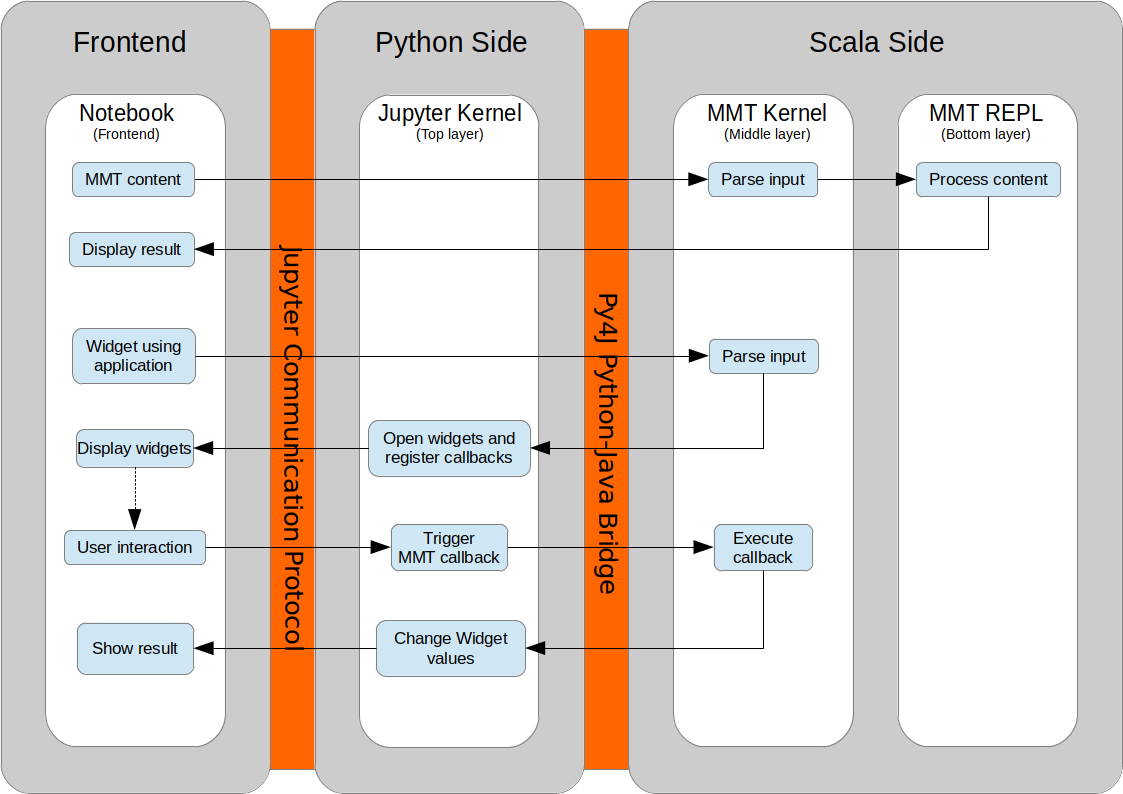
\includegraphics[width=12cm]{figures/ArchitectureDiagram}
  \caption{
    Architecture diagram.
    Steps that simply forward data from one layer to the next are not shown explicitly. 
  }\label{fig:architecture-diagram}
\end{figure}


Figure~\ref{fig:architecture-diagram} shows the details of the communication.
The upper part shows the simplest (widget-less) case: MMT content is entered in the frontend and forwarded to the bottom layer, and the response is forwarded in the opposite direction. 

The lower part shows a more complex widget-based interaction.
First of all, we add special management commands that are not passed on to the GUI-agnostic bottom layer.
Instead, they are identified by the middle layer, which responds by delegating to a GUI application.
This application then builds its graphical interface by calling the callbacks passed along by the top layer.
This results in a widget object in Python that is returned to the top layer and then forwarded to the frontend.

As usual, GUI components may themselves carry callback functions for handling events that are triggered by user interaction with the GUI in the frontend.
While conceptually straightforward, this leads to an unusually deep nesting of cross-programming language callbacks.
When creating a widget, the Scala-based GUI application may pass Scala callbacks whose implementation makes use of the callbacks provided by the top layer.
Thus, a user interaction triggers an MMT callback in the Python top layer, which is executed on the Scala side via Py4J, which in turn may call the Python callbacks exposed via Py4J.

\paragraph*{Example: In-Document Computation}

\begin{wrapfigure}{r}{0.5\textwidth}
  \vspace{-10pt}
  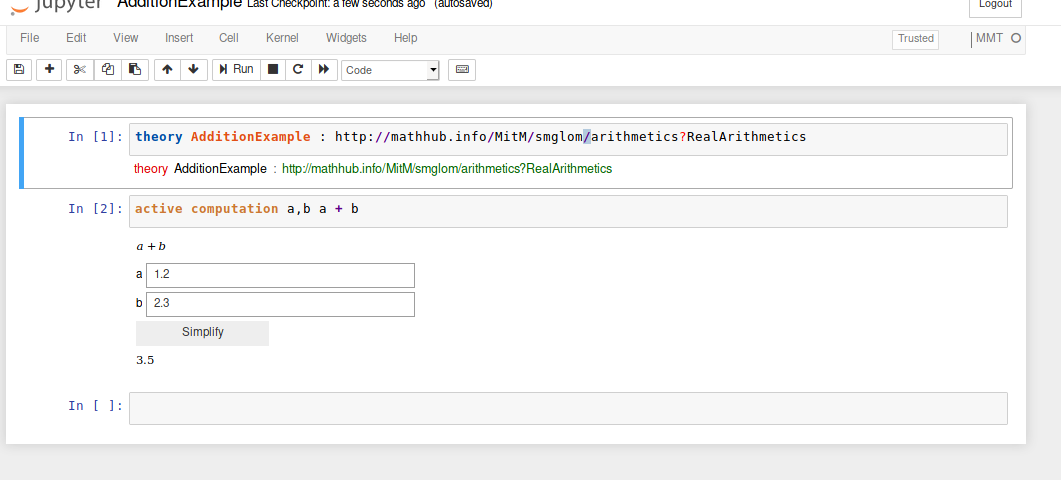
\includegraphics[width=0.5\textwidth]{screenshots/activecomp}
  \caption{An Active Computation widget in a Notebook via Jupyter/MMT Widgets}\label{fig:ac}
  \vspace{-20pt}
\end{wrapfigure}
We present an example of a GUI application inside of a notebook. 
It can be seen in Figure~\ref{fig:ac}.
We will later use this widget for active in-document computation. 

This notebook first defines a new theory (in \texttt{In[1]}), called AdditionExample.
This theory makes use of the MMT implementation of real number arithmetics.  

Our widget is then triggered in \texttt{In[2]} by the special command \texttt{active computation}. 
It takes two parameters, a list of variables (here $a$ and $b$) and a term (here $a + b$). 

These parameters are sent to the middle layer of our MMT kernel (see again Figure~\ref{fig:architecture-diagram}). 
This Scala code then parses the parameters (using the bottom layer), and instructs the middle layer to create a label and a text field for each variable. 
Furthermore, it also instructs the python code to create a button labeled \texttt{Simplify} and registers a callback inside the Scala code to be executed when the button is pressed. 
The labels, input fields and the button being used here are standard Jupyter widgets. 

In our case the user has already entered some terms, $1.2$ for $a$ and $2.3$ for $b$, and already clicked the \texttt{Simplify} button. 
This triggered the previously registered callback in the middle layer. 
The function first used the bottom layer to parse the terms inside the input fields. 
It then substituted the results into the original term $a + b$. 
The result of this substiution (in this case $1.2 + 2.3$) was then simplified (again using bottom layer code). 
This resulted in the final output of $3.5$. 

The important take-away here is not the difficulty of the computation\footnote{
  In our current implementation we compute using MMT. 
  MMT models computation using term simplfication. 
  However in principle it is possible to use any kind of computation engine here. 
  We want to integrate the active computation widget with our work on the Math-In-The-Middle CITATION paradigm which would be ideally suited for further applications. 
}\ednote{CITATION wp6-report}; it is the seamless integration between the frontend, top, middle and bottom layer code. 
This example demonstrates that our design makes it very easy to build and deploy simple GUI applications for MMT --- we still have the full power of Jupyter widgets at our fingertips. 

%%% Local Variables:
%%% mode: latex
%%% mode: visual-line
%%% fill-column: 5000
%%% TeX-master: "paper"
%%% End:

%  LocalWords:  Jupyter newpart textbf ednote centering texttt includegraphics synchronized customizable inparaenum Realizing subsubsection serialized emph emph emphasizes xeus xwidgets textit activecomp synchronization
